\chapter{Clystyru $k$-cymedr}\label{cha:literature}
\section{Cefndir}\label{sec:axelrodoriginal}
Mae clystyru $k$-cymedr yn ffordd o ddysgu heb oruchwyliaeth, mae'n cymryd data heb ei labelu ac yn eu sortio i mewn i $k$ wahanol glystyrau yn yr obaith i ddarganfod rhyw strwythur doedden ddim yn gwybod gynharach.

\begin{figure}
\begin{center}
\begin{minipage}{.4\linewidth}
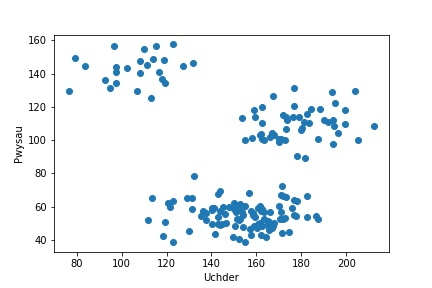
\includegraphics[width=1\linewidth]{../img/Scatterpython.jpeg}
\end{minipage}%
\begin{minipage}{1cm}
$\Rightarrow$
\end{minipage}%
\begin{minipage}{.4\linewidth}
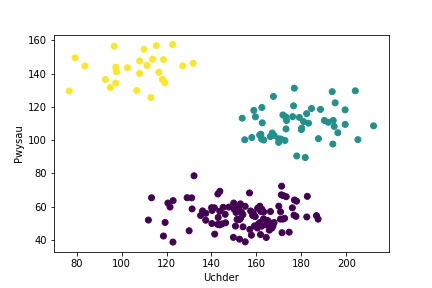
\includegraphics[width=1\linewidth]{../img/3clystwrpython.jpeg}
\end{minipage}%
\label{fig:Cefndir_Clysteru_k_modd}
\caption{Cyn ac ar \^{o}l clystyru $k$-cymedr.}
\end{center}
\end{figure}

I roi enghraifft i'r llun uchod, mae'r gwerthoedd ar echelin $x$ yn cynrychioli uchder rhyw berson ag yr llall yn cynrychioli pwysau'r person. Fel gwelwn yn Ddarlun~\ref{fig:Cefndir_Clysteru_k_modd} gallwn weld tri gr\^{w}p naturiol wedi'i ffurfio. Rydym nawr eisiau eu grwpio yn ffurf Fathemategol. Fysa clystyru $k$-cymedr medru dosrannu'r tri gr\^{w}p fel gwelwn ar ochr dde'r darlun. 

%%Adio mwy ar sut a pam mae'n cael ei ddefnyddio..

\section{Sut mae Clystyru $K$-cymedr yn gweithio?}

\subsection{Y Dull}

Mae clystyru $k$-cymedr yn syml, mae dim ond yn dilyn pedwar cam \cite{K-means-clustering}. I wneud yn si\^{w}r fod yn ei ffurf fwyaf cyntefig, fyddan yn defnyddio mesur pellter Ewclidaidd. Yn ogystal fydd rhaid dewis $k$ cyn cychwyn y proses. Mae'n bosib optimeiddio'r dewis o $k$, wnawn drafod am hyn hwyrach ymlaen. Dyma pedwar cam yr algorithm a sut fyddem yn edrych pan fyddwn ni yn ei ymgeisio'r algorithm ar y data welwn yn \ref{fig:Cefndir_Clysteru_k_modd}:

\begin{enumerate}
\item Aseinio pob elfen i un o'r $k$ clystyrau ar hap.

\begin{figure}[H]
\begin{center}
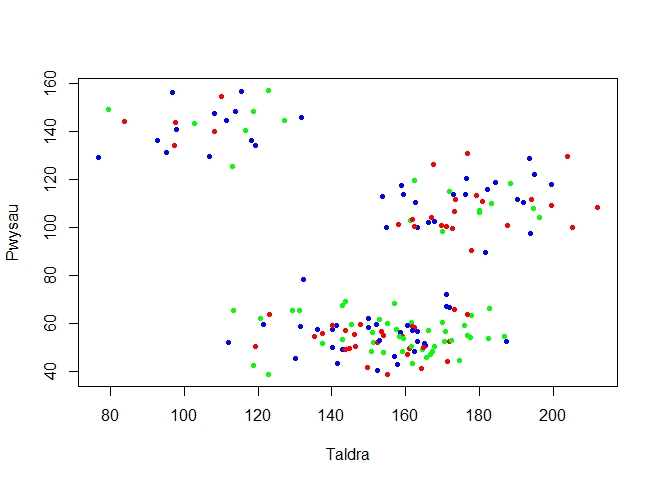
\includegraphics[width=0.5\linewidth]{../img/Cam1.jpeg}
\end{center}
\end{figure}

\item Cyfrifo'r cymedr pob clwstwr.

\begin{figure}[H]
\begin{center}
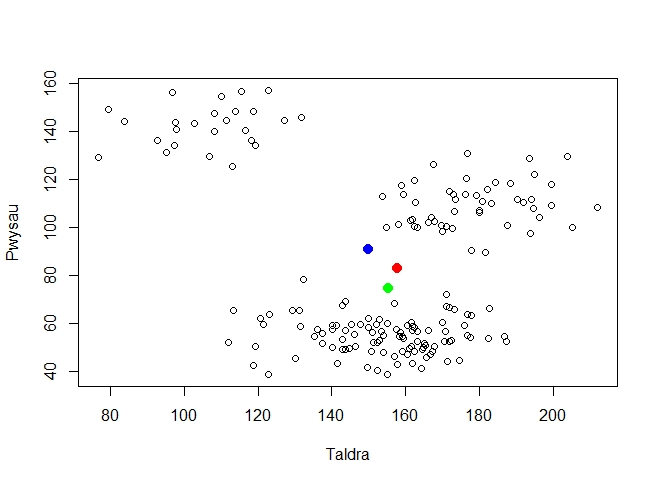
\includegraphics[width=0.5\linewidth]{../img/ClystyrauCychwynol.jpeg}
\end{center}
\end{figure}

\item Aseinio pob elfen unwaith eto i'r clwstwr gyda chymedr agosaf.

\begin{figure}[H]
\begin{center}
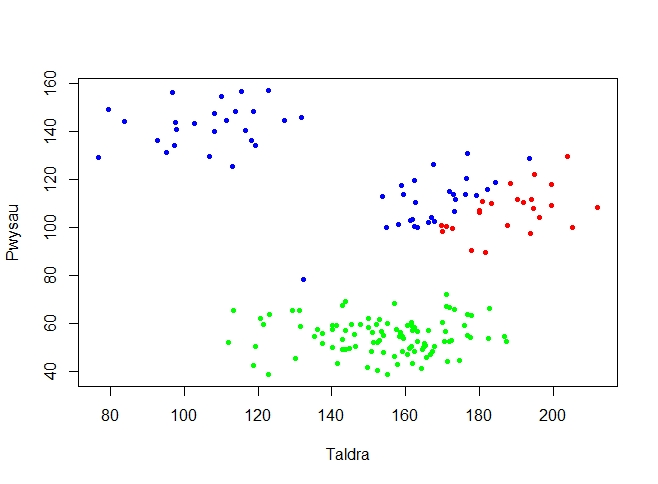
\includegraphics[width=0.5\linewidth]{../img/Cam3.jpeg}
\end{center}
\end{figure}

\item Ailadrodd camau dau a tri tan fod y creiddiau ddim yn symud unrhyw mwy.

\begin{figure}[H]
\begin{center}
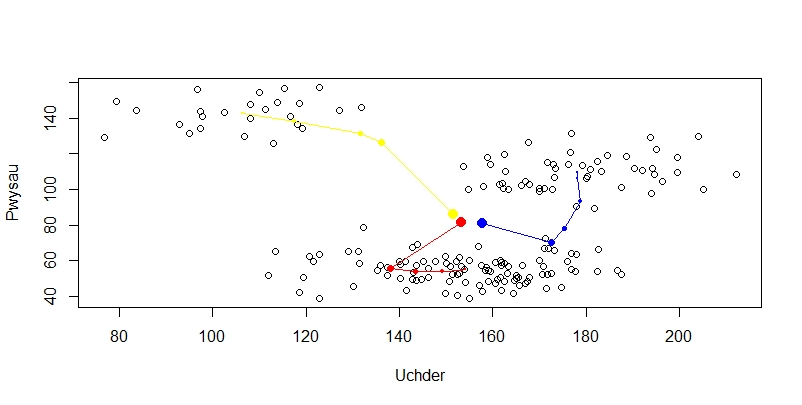
\includegraphics[width=0.5\linewidth]{../img/Convergence4.jpeg}
\end{center}
\end{figure}

\end{enumerate}  

\subsection{Darn Mathemategol}

Diffiniwn bob clwstwr rydym yn ceisio darganfod fel $C_i$ lle bydd i $\in \{ 1, 2, \dots, k\}$, mae gennym hefyd $n$ pwyntiau data $x_1,x_2,\dots,x_n$. Y darn gyntaf fydd i aseinio pob $x_j$ i ryw glwstwr $C_i$ ar hap. Yna gan ein bod yn datgelu ein bod yn delio gyda phl\^{a}n Ewclidaidd, mi fyddem yn delio gyda darganfod cymedr pob clwstwr gan y fformiwla ganlynol:
Diffiniwn $S_i$ fel y set o bwyntiau data sydd wedi'i aseinio i glwstwr $C_i$.
$$ C_i = \frac{1}{|S_i|}\sum_{x_j \in S_i} {x_j} $$
Nawr mae pob clwstwr gyda chymedr newydd, fedrem aseinio pob pwynt data i'r craidd agosaf. Fydd hyn yn cael ei gwneud gan fynd drwy bob pwynt data ag cyfrifo'r pellter Ewclidaidd i bob craidd. Yna fydd y pwynt priodol yn cael ei labelu gyda'r clwstwr gyda phellter lleiaf o'r craidd i'r pwynt data.
$$ \arg \min_{c_i} dist(c_i,x_j)^2$$
Unwaith mae'r proses wedi'i chychwyn, does dim ond angen ailadrodd y darn o ddarganfod y creiddiau newydd ag yna ail labelu'r pwyntiau data.


\subsection{Sut i ddarganfod y $K$ orau?}

Mae yna wahanol ffurf i ddarganfod $K$, wnawn edrych ar ddau wahanol ffordd o wneud hyn. 

\subsubsection{Dull Penelin}

Mae'r dull penelin yn cymharu'r cyfanswm o swm sgwariau o fewn y clystyrau. Unwaith gennym y cyfanswm o swm sgwariau o fewn clystyrau i bob $k$ rydym eisiau cymharu; fyddem yn creu plot o bob $k$ yn erbyn eu cyfanswm o swm sgwariau o fewn y clystyrau. Unwaith mae gennym y graff, allwn ei ddadansoddi. 

\begin{figure}[H]
\begin{center}
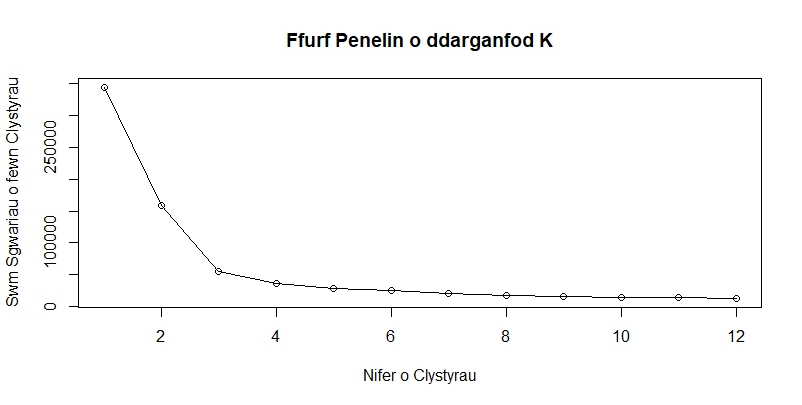
\includegraphics[width=0.5\linewidth]{../img/Dull_Penelin.jpeg}
\end{center}
\end{figure}

Yn y graff uchod sydd gennym, fydd yn dangos sut mae'r swm sgwariau yn fawr yn cychwyn gyda $k$=1 sydd yn gwneud synnwyr. O'r pwynt yma wedyn fydd yna newid ystyrlon yn y swm sgwariau. Unwaith mae'r newid ystyrlon yn dod i ben fydd gennym ongl yn cael ei greu lle bydd newid $K$ dim ond yn creu newid ymylol. Y pwynt yma fydd yr optimwm nifer o $K$. Fel gwelwn yn glir yn ein henghraifft ni, mae'n glir fod $K$=3 yw dewis orau ar $K$.

\subsubsection{Dendrogram}

Mae Dendrogram yn fath wahanol iawn i dangos y nifer orau o $k$. Mae'n defnyddio darn o glystyru hierarchaidd i greu diagram canghennog. Mae'r echelin llorweddol yn dangos phob gwrthrych yn ein set o ddata. Mae'r echelin fertigol yn dangos annhebygrwydd. Ar gyfer yr un data, casglon ni:

\begin{figure}[H]
\begin{center}
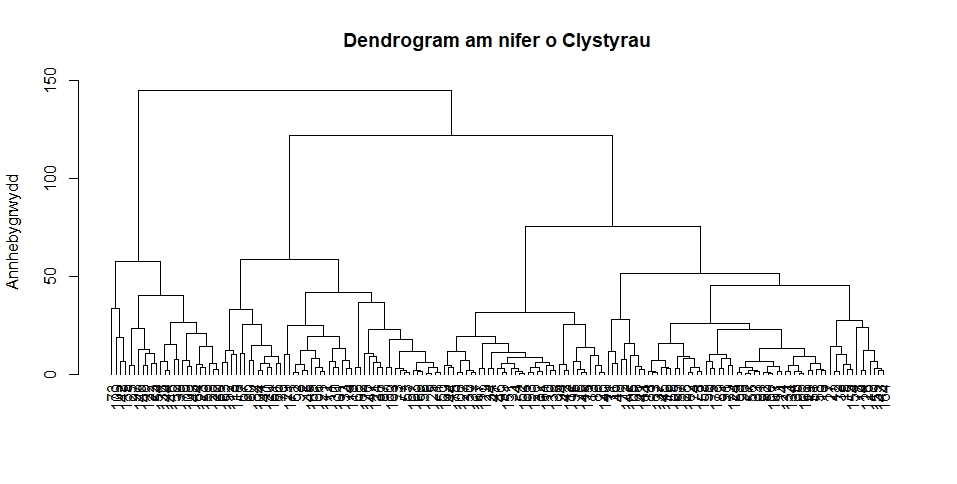
\includegraphics[width=0.5\linewidth]{../img/Dendrogram.jpeg}
\end{center}
\end{figure}

I ddadansoddi'r Dendrogram mi fyddwn edrych yn bennaf ar yr echelin fertigol. Edrychem allan am y fwyaf annhebygrwydd rhwng cyflwyniad o gangen arall yn y goeden. Welwn ni hyn yn ein henghraifft ni ar \^{o}l i'r drydydd clwstwr cael ei gyflwyno yn dendrogram. Mae hyn yn datganu'r un peth a'r dull penelin.

\section{Tiwtorial yn R}
Mi fyddwn yn edrych ar ddata o uchder a phwysau 175 wahanol berson. Mi allwch chi lawrlwytho y data yma o fan hyn. 

Yno fydd angen lawrlwytho a gosod y pecynnau "graphics", "stats" ag "datasets" ar eich fersiwn chi o R studio. Ffordd hawdd i wirio hyn fydd i ddefnyddio'r c\^{o}d canlynol:

\begin{minted}{r}
install.packages("graphics")
install.packages("stats")
install.packages("datasets")
library(graphics)
library(stats)
library(datasets)
\end{minted}
Mae'r darn gyntaf o'r c\^{o}d uchod yn gosod/diweddaru y pecynnau angenrheidiol. Mae'r ail ddarn yn llwytho'r pecynnau i ein fersiwn ni o R Studio.

Nawr mi wnawn fewnforio'r data. 

\begin{minted}{r}
heightvsweight <- read.csv("C:/Users/User/Desktop/Dysgu_Peirianyddol/heightvsweight.csv")
View(heightvsweight)
\end{minted}

Fydd rhaid gwneud yn si\^{w}r fod eich cyfeiriadur yn gywir i'r lleoliad o eich ffeil chi.
Ar \^{o}l rhedeg y c\^{o}d ddylai tabl agor mewn tab arwahan. Ddylai edrych yn debyg i'r canlynol:

\begin{figure}[H]
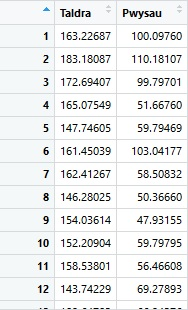
\includegraphics[width=0.35\linewidth]{../img/Data_yn_R.jpg}
\label{fig:DataR}
\end{figure}

Gan fod y data hefo enwau ar gyfer y colofnau, gallwn atodi'r data i lwybr chwilio R. Bydd hyn yn gadael i ni gyfeirio at enwau colofnau'r data yn ein c\^{o}d fydd yn gwneud yn lawer mwy symlach i ddeall.

\begin{minted}{r}
attach(heightvsweight)
\end{minted}

I wneud fwy o synnwyr o'r data, mi wnawn blotio'r data. Wnawn weld fod yna 3 clwstwr clir. 

\begin{minted}{r}
plot(Uchder, Pwysau, pch = 21)
\end{minted}

\begin{figure}[H]
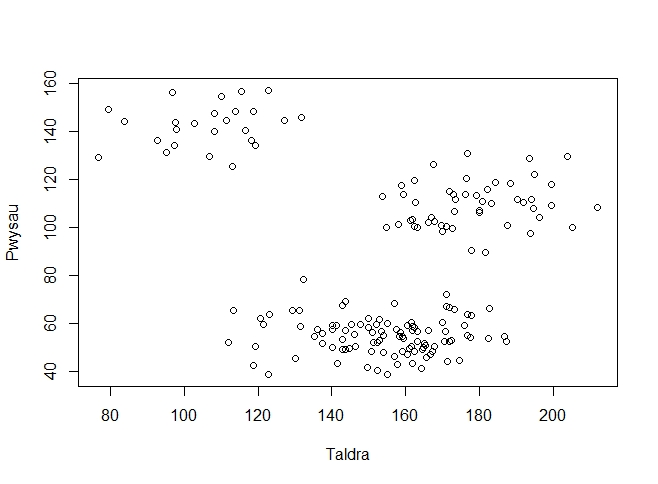
\includegraphics[width=0.5\linewidth]{../img/ScatterplotR.jpeg}
\label{fig:ScatterplotR}
\end{figure}

R\^{w}an rydym yn gallu gweld fod y data yn gallu cael i rannu i dri chlwstwr gwahanol, mi wnawn ddefnyddio y ffurf Fathemategol i'w ddehongli. Rhedwn y canlynol i redeg clystyru $k$-cymedr yn R. Rydym yn defnyddio'r ymresymiad "nstart" i ddewis faint o setiau ar hap o greiddiau wnawn gymered.

\begin{minted}{r}
kcymedr <- kmeans(heightvsweight,3, nstart = 50)
\end{minted}

Allwn nawr adio colofn newydd i'r data sef y clystyrau newydd mae'r algorithm wedi'i darganfod.

\begin{minted}{r}
heightvsweight$Clwstwr3 <- kcymedr$cluster
\end{minted}

Gallwn weld y newid hwn gan ddefnyddio'r c\^{o}d o gynnar.

\begin{minted}{r}
View(heightvsweight)
\end{minted}

\begin{figure}[H]
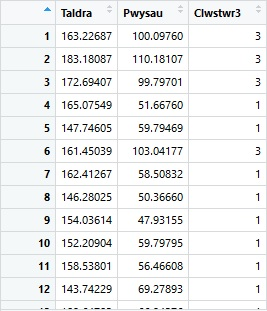
\includegraphics[width=0.5\linewidth]{../img/Data3_yn_R.jpg}
\end{figure}

Mae'n bosib fydd yr algorithm wedi rhoi rhif gwahanol ar gyfer clystyrau gwahanol ond ddylai'r clystyrau fod yn hafal. Mae hyn oherwydd y setiau ar hap mae'r fformiwla yn ei gymered yn cychwyn.

Rhedwn y c\^{o}d canlynol i gael gweld y clystyrau newydd ar graff.

\begin{minted}{r}
plot(Uchder, Pwysau, pch = 21, bg=c("red","green","blue")[unclass(kcymedr$cluster)])
\end{minted}

\begin{figure}[H]
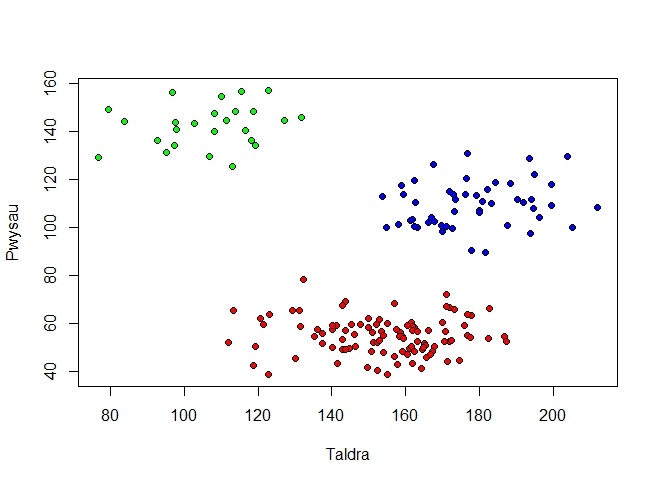
\includegraphics[width=0.5\linewidth]{../img/3clwstwrR.jpeg}
\end{figure}

Y nawr mi nawn rhedeg yr algorithm ar gyfer 6 clwstwr i weld y clystyrau pan fydd $k$=6. 

\begin{minted}{r}
kcymedr <- kmeans(heightvsweight,6, nstart = 50)
heightvsweight$Clwstwr6 <- kcymedr$cluster
View(heightvsweight)
\end{minted}

\begin{figure}[H]
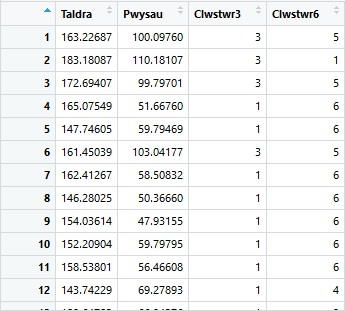
\includegraphics[width=0.5\linewidth]{../img/Data6_yn_R.jpg}
\end{figure}

Gwelwn fod yr labelau newydd wedi cael ei ychwanegu i ein tabl. Yna gan blotio graff arall, fedrem weld y 6 clwstwr yn gliriach.

\begin{minted}{r}
plot(Uchder, Pwysau, pch = 21, bg=c("red","green","blue", "yellow", "black", "white")[unclass(kcymedr$cluster)])
\end{minted}

\begin{figure}[H]
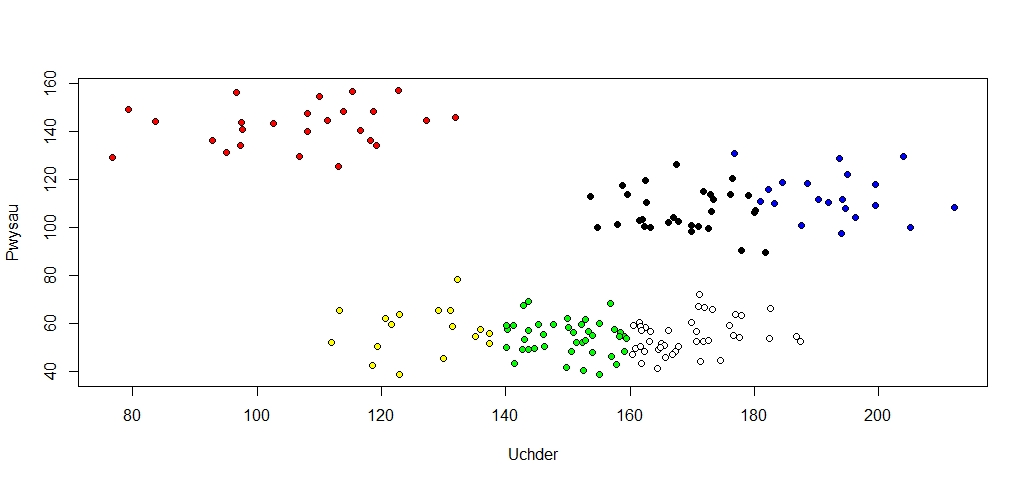
\includegraphics[width=0.5\linewidth]{../img/6clwstwrR.jpeg}
\end{figure}


%Mae'r data iris ar gael iddym drwy'r pecyn "datasets". Yn yr enghraifft top mi wnaethom defnyddio k fel 3, felly hyna be wnawn neud eto.
%Dyma'r c\^{o}d ar gyfer rhedeg clystyru k-cymedr:
%\begin{minted}{r}
%clysteru_tri <- kmeans(iris[,1:4],3, nstart = 20)
%clysteru_tri 
%\end{minted}
%Mae'r llinell gyntaf o c\^{o}d yn rhedeg clystyru k-cymedr ar y set data iris gyda k=3. Mae'r darn nstart yn cynrychioli faint o dosraniadau i drio yn cychwyn yn erbyn'r ffwythiant amcan, er mwyn dewis y cychwyn orau. Mae'r ail linell yn allbwn yr wybodaeth canlynol:
%\begin{minted}{r}
%>>>K-means clustering with 3 clusters of sizes 50, 62, 38
%>>>
%>>>Cluster means:
%>>>  Sepal.Length Sepal.Width Petal.Length
%>>>1     5.006000    3.428000     1.462000
%>>>2     5.901613    2.748387     4.393548
%>>>3     6.850000    3.073684     5.742105
%>>>  Petal.Width
%>>>1    0.246000
%>>>2    1.433871
%>>>3    2.071053
%>>>
%>>>Clustering vector:
%>>>  [1] 1 1 1 1 1 1 1 1 1 1 1 1 1 1 1 1 1 1 1 1 1 1
%>>> [23] 1 1 1 1 1 1 1 1 1 1 1 1 1 1 1 1 1 1 1 1 1 1
%>>> [45] 1 1 1 1 1 1 2 2 3 2 2 2 2 2 2 2 2 2 2 2 2 2
%>>> [67] 2 2 2 2 2 2 2 2 2 2 2 3 2 2 2 2 2 2 2 2 2 2
%>>> [89] 2 2 2 2 2 2 2 2 2 2 2 2 3 2 3 3 3 3 2 3 3 3
%>>>[111] 3 3 3 2 2 3 3 3 3 2 3 2 3 2 3 3 2 2 3 3 3 3
%>>>[133] 3 2 3 3 3 3 2 3 3 3 2 3 3 3 2 3 3 2
%>>>
%>>>Within cluster sum of squares by cluster:
%>>>[1] 15.15100 39.82097 23.87947
%>>> (between_SS / total_SS =  88.4 %)
%\end{minted}
%Mae'r c\^{o}d uchod rhoi pob wybodaeth a fysa chi eisiau wybod fel allbwn o'r proses.
%I weld y clysterau allwn plotio graff ar gyfer phob cyfuniad o newidynnau. Mae hyn yn alluogi ni i weld yr gwaith dpsbarthu mae'r algorithm wedi'i neud.
%\begin{minted}{r}
%plot(iris[,1:4], pch = 24, bg=c("red","green3","blue")[unclass(clysteru_tri$cluster)])
%\end{minted}
%Yn y ffwythiant "plot" uchod, mae'r darn gynta ohono yn cyfeirio tuag at pa data fydd yn cael ei clysteru. Mae'r ail darn yn penodi be fydd pob pwynt data yn cael ei cynrychioli fel pan %mae'r darn dwythaf yn penodi lliw i pob clwstwr.

%Mi wnawn edrych y nawr ar yr set data iris sy'n boblogaidd iawn yn y maes ystadegaeth a gwyddor data. Mae'r data yn cynnwys mesuriadau uchder ag lled petal a setal 150 planhigyn iris. Yn isod gweler lun o allbwn clystyru k-cymedr yn erbyn y clystyrau gwreiddiol o'r data. Gwelwyd fod yr algorithm yn neud yn wych!


\section{Tiwtorial yn python}
Yn y tiwtorial hwn mi wnawn edrych ar yr un data a welom yn y tiwtorial diwethaf.
I gychwyn bydd rhaid mewnforio'r pecynnau pandas, matplotlib.pyplot ag sklearn.cluster drwy redeg y c\^{o}d canlynol:

\begin{minted}{python}
import pandas as pd
import matplotlib.pyplot as plt
import sklearn.cluster
\end{minted}

Y r\^{w}an mi wnawn fewnforio'r data i mewn i ein gwaith gan redeg y c\^{o}d:
\begin{minted}{python}
data = pd.read_csv('heightvsweight.csv')
\end{minted}
Fydd rhaid gwneud yn si\^{w}r fod y data wedi cael ei gadw yn yr un cyfeiriadur ag y ffeil rydych yn ei ddefnyddio i redeg y c\^{o}d.
Unwaith fydd wedi cael ei mewnforio, allwn ni gweld yn fras y data gennym ni. 
\begin{minted}{python}
data.head()
\end{minted}

\begin{figure}
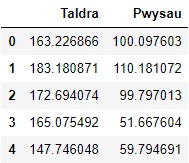
\includegraphics[width=0.35\linewidth]{../img/tabl1.jpg}
\label{fig:Data1}
\end{figure}

I weld y data mewn ffordd fwy gweledol, wnawn blotio graff gwasgariad o'r data

\begin{minted}{python}
plt.scatter(data['Uchder'], data['Pwysau']);
plt.xlabel('Uchder')
plt.ylabel('Pwysau')
plt.show()
\end{minted}

\begin{figure}[H]
\begin{center}
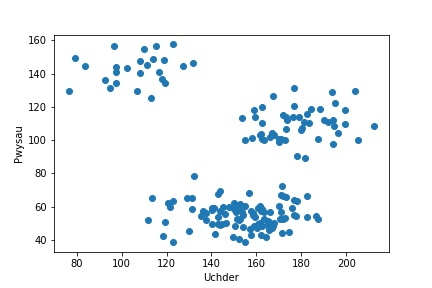
\includegraphics[width=0.7\linewidth]{../img/Scatterpython.jpeg}
\caption{Enghraifft o ddata da i cael ei clystyru.}
\label{fig:Scatterpython}
\end{center}
\end{figure}

Fel gwelwn, mae'r data yn edrych fel ei fod mewn tri chlwstwr. Felly wnawn ddefnyddio'r ffurf Fathemategol i ddarparu arnyn nhw.

\begin{minted}{python}
kmeans = sklearn.cluster.KMeans(n_clusters=3).fit(data)
data['Cluster (k=3)'] = kmeans.predict(data)
\end{minted}



\begin{minted}{python}
data.head()
\end{minted}

\begin{figure}[H]
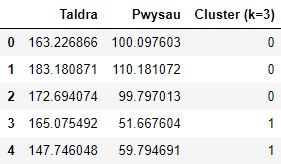
\includegraphics[width=0.35\linewidth]{../img/tabl2.jpg}
\label{fig:Data2}
\end{figure}

Fel y gwelwyd, mae'r data wedi'i rhoi i mewn clwstwr ac wedi'i labelu gyda rhif y clwstwr. Gan fod pob pwynt yn y data nawr gyda label, allwn ni creu'r plot eto ond gyda bob clwstwr yn lliw gwahanol.

\begin{minted}{python}
plt.scatter(data['Uchder'], data['Pwysau'], c=data['Cluster (k=3)']);
plt.xlabel('Uchder')
plt.ylabel('Pwysau')
plt.show()
\end{minted}

\begin{figure}[H]
\begin{center}
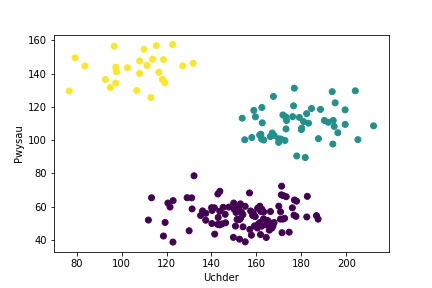
\includegraphics[width=0.7\linewidth]{../img/3clystwrpython.jpeg}
\caption{Sut ddylsa eich graff edrych gyda 3 clystwr.}
\label{fig:3clystwrpython}
\end{center}
\end{figure}

Fel y gwelwn, gweithiodd yr algorithm yn wych, wnawn nawr trio clystyru $k$-cymedr gyda $k$ yn hafal i 6.

\begin{minted}{python}
kmeans = sklearn.cluster.KMeans(n_clusters=6).fit(data)
data['Cluster (k=6)'] = kmeans.predict(data)
\end{minted}

\begin{minted}{python}
data.head()
\end{minted}

\begin{figure}[H]
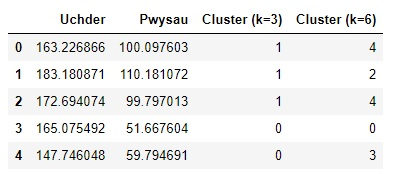
\includegraphics[width=0.35\linewidth]{../img/tabl3.jpg}
\label{fig:Data3}
\end{figure}

Gwelwn caiff y data yn ogystal ei rhoi i mewn i 6 clwstwr gwahanol. 

\begin{minted}{python}
plt.scatter(data['Uchder'], data['Pwysau'], c=data['Cluster (k=6)']);
plt.xlabel('Uchder')
plt.ylabel('Pwysau')
plt.show()
\end{minted}

\begin{figure}[H]
\begin{center}
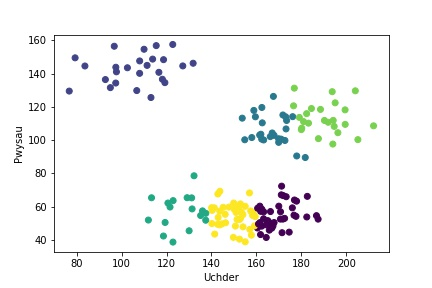
\includegraphics[width=0.7\linewidth]{../img/6clystwrpython.jpeg}
\caption{Sut ddylsa eich graff edrych gyda 6 clystwr.}
\label{fig:6clystwrpython}
\end{center}
\end{figure}

Dyma sut dylaf eich data edrych fel ar \^{o}l a phrosesu drwy glystyru 6-cymedr. 